\documentclass[9pt,a4paper]{extarticle}
\usepackage{parskip}

\usepackage[utf8]{inputenc}
\usepackage[T1]{fontenc}
\usepackage[portuguese]{babel}
\usepackage{amsmath, amssymb, amsthm}
\usepackage{geometry}
\usepackage{listings}
\usepackage{xcolor}
\usepackage{hyperref}
\usepackage{booktabs}
\usepackage{array}
\usepackage{tabularx}
\usepackage{enumitem}
\usepackage[expansion=false]{microtype}
\usepackage{csquotes}
\usepackage{natbib}
\usepackage{algorithm}
\usepackage{algpseudocode}
\usepackage{tikz}
\usetikzlibrary{positioning}

\definecolor{important}{RGB}{255, 100, 100}
\definecolor{notice}{RGB}{0, 102, 204}

\newcommand{\impt}[1]{\textcolor{important}{#1}}
\newcommand{\ntc}[1]{\textcolor{notice}{#1}}

\setlist{nosep}
\geometry{margin=2cm}

\newtheorem{theorem}{Teorema}[section]
\newtheorem{lemma}[theorem]{Lema}
\newtheorem{corollary}[theorem]{Corolário}
\newtheorem{proposition}[theorem]{Proposição}
\theoremstyle{definition}
\newtheorem{definition}{Definição}[section]
\newtheorem{example}{Exemplo}[section]
\newtheorem{remark}{Observação}[section]

% Personalização do algpseudocode
\algrenewcommand\algorithmicrequire{\textbf{Entrada:}}
\algrenewcommand\algorithmicensure{\textbf{Saída:}}
\algrenewcommand\algorithmicwhile{\textbf{enquanto}}
\algrenewcommand\algorithmicdo{\textbf{faça}}
\algrenewcommand\algorithmicif{\textbf{se}}
\algrenewcommand\algorithmicthen{\textbf{então}}
\algrenewcommand\algorithmicelse{\textbf{senão}}
\algrenewcommand\algorithmicfor{\textbf{para}}
\algrenewcommand\algorithmicreturn{\textbf{retorna}}
\algrenewcommand\algorithmicend{\textbf{fim}}

\title{Heapsort e Quicksort\footnote{Material baseado em \citep{cormen2009}.}}
\author{PCC104 -- Projeto e Análise de Algoritmos}
\date{\today}

\begin{document}
\maketitle
\tableofcontents

% =====================================================================
\section{Introdução}

Nesta aula estudamos dois algoritmos de ordenação por comparação que,
embora compartilhem o tempo assintótico $O(n\lg n)$ com o \textit{merge sort},
apresentam propriedades bastante distintas:

\begin{itemize}
  \item \impt{Heapsort:} ordena \textit{in place} e garante $O(n\lg n)$ no
    \textbf{pior caso}. A ideia central é uma estrutura de dados implícita --- o
    \textit{heap} --- que mantém uma ordem parcial sobre os elementos.
  \item \impt{Quicksort:} ordena \textit{in place}, tem tempo $\Theta(n^2)$
    no pior caso, mas seu \textbf{caso médio é $O(n\lg n)$} com constantes
    muito pequenas. Na prática, é o mais rápido dos três para entradas
    grandes e aleatórias.
\end{itemize}

\ntc{Ambos os algoritmos são comparativos:} assumimos apenas que os elementos
admitem uma relação de ordem total e que podemos testá-la com operações de
comparação.

% =====================================================================
\section{Heapsort}

\subsection{A estrutura de dados \textit{heap}}

\begin{definition}[Heap binário como arranjo]\label{def:heap}
Um \impt{heap binário} é um arranjo $A[1\mathinner{.\,.} n]$ que visualizamos como
uma árvore binária quase completa, preenchida da esquerda para a direita.
Para um nó de índice $i$, definimos:
\[
  \textsc{Parent}(i) = \lfloor i/2 \rfloor, \qquad
  \textsc{Left}(i) = 2i, \qquad
  \textsc{Right}(i) = 2i+1.
\]
\end{definition}

Dois atributos acompanham o arranjo: \texttt{A.length}, o número de posições
alocadas, e \texttt{A.heap-size}, o número de elementos válidos do heap
(sempre $\texttt{A.heap-size} \le \texttt{A.length}$).

\begin{definition}[Propriedade de \textit{max-heap}]
Um arranjo $A$ satisfaz a \impt{propriedade de max-heap} se, para todo
índice $i > 1$,
\[
  A[\textsc{Parent}(i)] \ge A[i].
\]
Equivalentemente, o valor de um nó não excede o valor de seu pai.
\end{definition}

\paragraph{Altura.} Definimos a altura de um nó como o número de arestas no
caminho descendente mais longo até uma folha; a altura do heap é a altura de
sua raiz. Como o heap é uma árvore binária quase completa, temos:

\begin{lemma}\label{lem:altura}
Um heap de $n$ elementos tem altura $\lfloor \lg n \rfloor$.
\end{lemma}

\begin{proof}
A árvore é quase completa, então todos os níveis $0, 1, \dots, h-1$ estão
cheios, totalizando $2^h - 1$ nós, e o nível $h$ tem entre $1$ e $2^h$ nós.
Assim $2^h \le n \le 2^{h+1} - 1$, o que dá $h = \lfloor \lg n \rfloor$.
\end{proof}

\ntc{Consequência direta:} operações que percorrem um caminho da raiz a uma
folha --- ou de uma folha à raiz --- custam $O(\lg n)$.

\begin{figure}[!ht]
  \centering
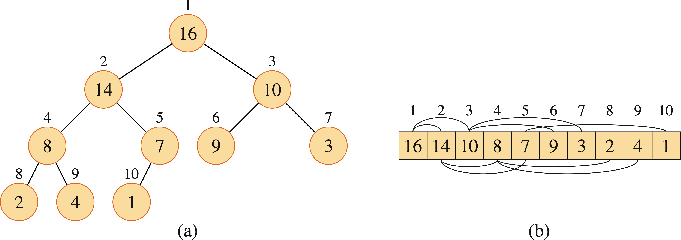
\includegraphics[width=0.7\textwidth]{Figure 6.1.pdf}
\caption{Estrutura de dados heap}
\end{figure}

\subsection{\textsc{Max-Heapify}: restaurando a propriedade de heap}

A operação \textsc{Max-Heapify} assume que as subárvores enraizadas em
\textsc{Left}$(i)$ e \textsc{Right}$(i)$ já são max-heaps, mas $A[i]$ pode
violar a propriedade localmente. O procedimento ``desce'' $A[i]$ pela
árvore até restaurar a propriedade.

\begin{algorithm}[H]
\caption{\textsc{Max-Heapify}$(A, i)$}
\begin{algorithmic}[1]
\State $\ell \gets \textsc{Left}(i)$
\State $r \gets \textsc{Right}(i)$
\If{$\ell \le A.\text{heap-size}$ \textbf{e} $A[\ell] > A[i]$}
  \State $\textit{largest} \gets \ell$
\Else
  \State $\textit{largest} \gets i$
\EndIf
\If{$r \le A.\text{heap-size}$ \textbf{e} $A[r] > A[\textit{largest}]$}
  \State $\textit{largest} \gets r$
\EndIf
\If{$\textit{largest} \ne i$}
  \State troca $A[i] \leftrightarrow A[\textit{largest}]$
  \State \textsc{Max-Heapify}$(A, \textit{largest})$
\EndIf
\end{algorithmic}
\end{algorithm}

\begin{figure}[!ht]
  \centering
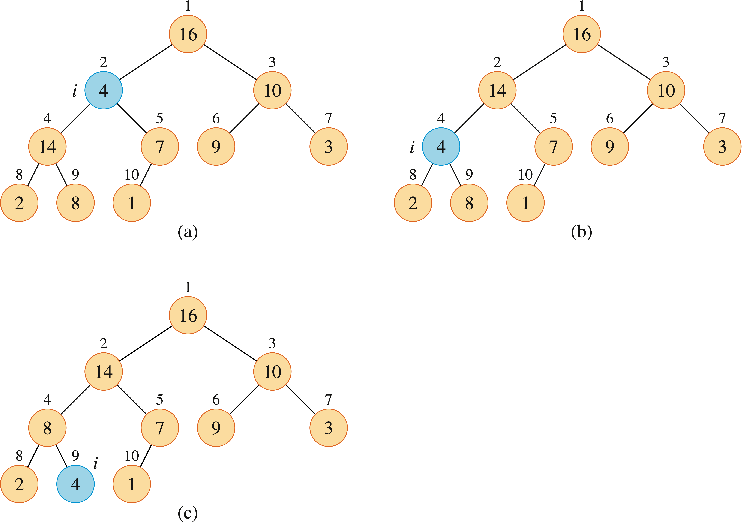
\includegraphics[width=0.7\textwidth]{Figure 6.2.pdf}
\caption{Execução Max-Heapify(A,2)}
\end{figure}

\begin{proposition}\label{prop:heapify}
O tempo de execução de \textsc{Max-Heapify} sobre um nó de altura $h$ é
$O(h)$; em particular, $O(\lg n)$ para o heap inteiro.
\end{proposition}

\begin{proof}
O trabalho local em cada chamada é $\Theta(1)$: comparações com os filhos
e, possivelmente, uma troca. A recursão desce por uma única subárvore, de
forma que
\[
  T(h) \le T(h-1) + \Theta(1),
\]
cuja solução é $T(h) = O(h)$. Como $h \le \lfloor \lg n\rfloor$
(Lema~\ref{lem:altura}), concluímos $T = O(\lg n)$.
\end{proof}

\begin{remark}
A recorrência que aparece no CLRS é $T(n) \le T(2n/3) + \Theta(1)$, onde o
fator $2/3$ corresponde ao tamanho máximo de uma subárvore filha em um heap
quase completo (pior caso quando o último nível está pela metade). Pelo
método mestre (caso 2), $T(n) = O(\lg n)$.
\end{remark}

\subsection{Construção do heap: \textsc{Build-Max-Heap}}

Dado um arranjo arbitrário, construímos um max-heap chamando
\textsc{Max-Heapify} nos nós internos, de baixo para cima. \impt{Nós nos
índices $\lfloor n/2\rfloor + 1, \dots, n$ são folhas} --- cada um é,
trivialmente, um max-heap unitário.

\begin{algorithm}[H]
\caption{\textsc{Build-Max-Heap}$(A)$}
\begin{algorithmic}[1]
\State $A.\text{heap-size} \gets A.\text{length}$
\For{$i \gets \lfloor A.\text{length}/2 \rfloor$ \textbf{até} $1$}
  \State \textsc{Max-Heapify}$(A, i)$
\EndFor
\end{algorithmic}
\end{algorithm}

\begin{figure}[!ht]
  \centering
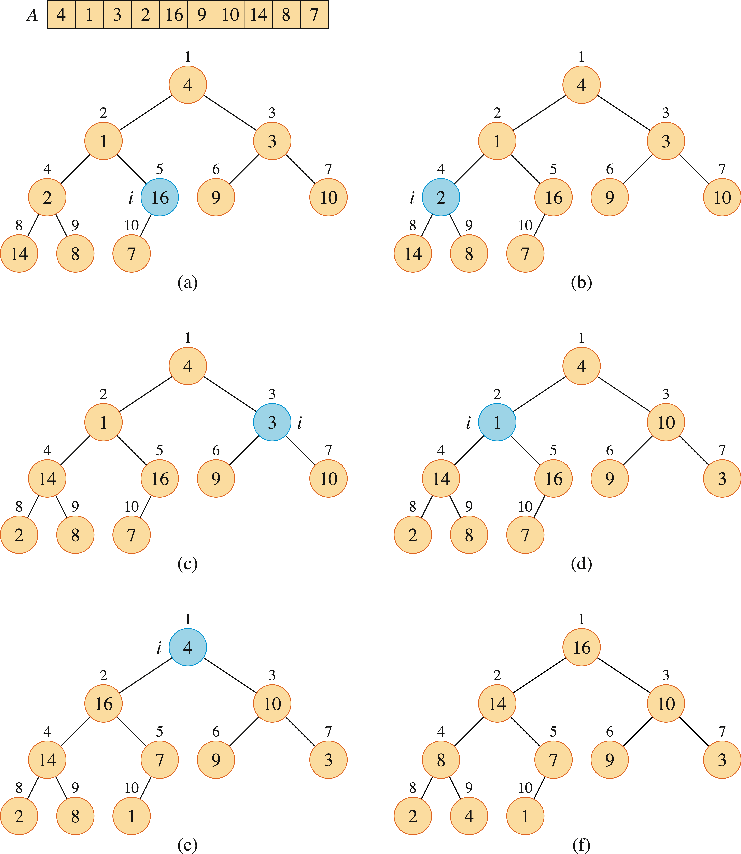
\includegraphics[width=0.7\textwidth]{Figure 6.3.pdf}
\caption{Execução Build-Max-Heap}
\end{figure}

\paragraph{Corretude (invariante de laço).} Antes da primeira iteração,
cada nó $\lfloor n/2\rfloor + 1, \dots, n$ é raiz de um max-heap (folhas).
Antes de cada iteração com índice $i$, cada nó $i+1, i+2, \dots, n$ é raiz
de um max-heap. A chamada \textsc{Max-Heapify}$(A, i)$ preserva essa
propriedade e estende-a a $i$. No fim, $i = 0$ e todo nó é raiz de um
max-heap, em particular $A[1]$.

\begin{theorem}\label{teo:build-heap}
\textsc{Build-Max-Heap} executa em tempo $O(n)$.
\end{theorem}

\begin{proof}
A análise ingênua dá $O(n\lg n)$: são $\Theta(n)$ chamadas, cada uma
$O(\lg n)$. Mas podemos apertar o limite observando que o custo de
\textsc{Max-Heapify} em um nó depende da \textit{altura} do nó, não de $n$.

Em um heap de $n$ elementos, o número de nós de altura $h$ é no máximo
$\lceil n/2^{h+1}\rceil$. Logo, o custo total é
\[
  T(n) \;=\; \sum_{h=0}^{\lfloor \lg n\rfloor}
            \Big\lceil \tfrac{n}{2^{h+1}}\Big\rceil \cdot O(h)
       \;=\; O\!\left( n \sum_{h=0}^{\lfloor \lg n\rfloor} \tfrac{h}{2^h}\right).
\]
Usando a identidade $\sum_{h=0}^{\infty} h/2^h = 2$, obtemos
$T(n) = O(n)$.
\end{proof}

\ntc{Ou seja:} construir o heap é \textbf{linear}. É um resultado
surpreendente à primeira vista, mas decorre do fato de que a grande
maioria dos nós está próxima das folhas, onde \textsc{Max-Heapify} custa
pouco.

A soma que aparece na análise de \textsc{Build-Max-Heap} é
\[
  \sum_{i=0}^{h} 2^i (h - i) = 2^{h+1} - h - 2.
\]

Como $h = \lfloor \lg n \rfloor$, temos $2^h \le n < 2^{h+1}$, logo
$2^{h+1} \le 2n$. Portanto
\[
  \sum_{i=0}^{h} 2^i (h - i) \;=\; 2^{h+1} - h - 2 \;\le\; 2n - \lfloor \lg n \rfloor - 2 \;=\; O(n).
\]

\subsection{O algoritmo \textsc{Heapsort}}

A ideia é simples: o máximo do arranjo está em $A[1]$. Trocamos $A[1]$
com $A[n]$, reduzimos o heap em uma unidade e restauramos a propriedade
chamando \textsc{Max-Heapify}. Repetimos até sobrar um único elemento.

\begin{algorithm}[H]
\caption{\textsc{Heapsort}$(A)$}
\begin{algorithmic}[1]
\State \textsc{Build-Max-Heap}$(A)$
\For{$i \gets A.\text{length}$ \textbf{até} $2$}
  \State troca $A[1] \leftrightarrow A[i]$
  \State $A.\text{heap-size} \gets A.\text{heap-size} - 1$
  \State \textsc{Max-Heapify}$(A, 1)$
\EndFor
\end{algorithmic}
\end{algorithm}

\begin{figure}[!ht]
  \centering
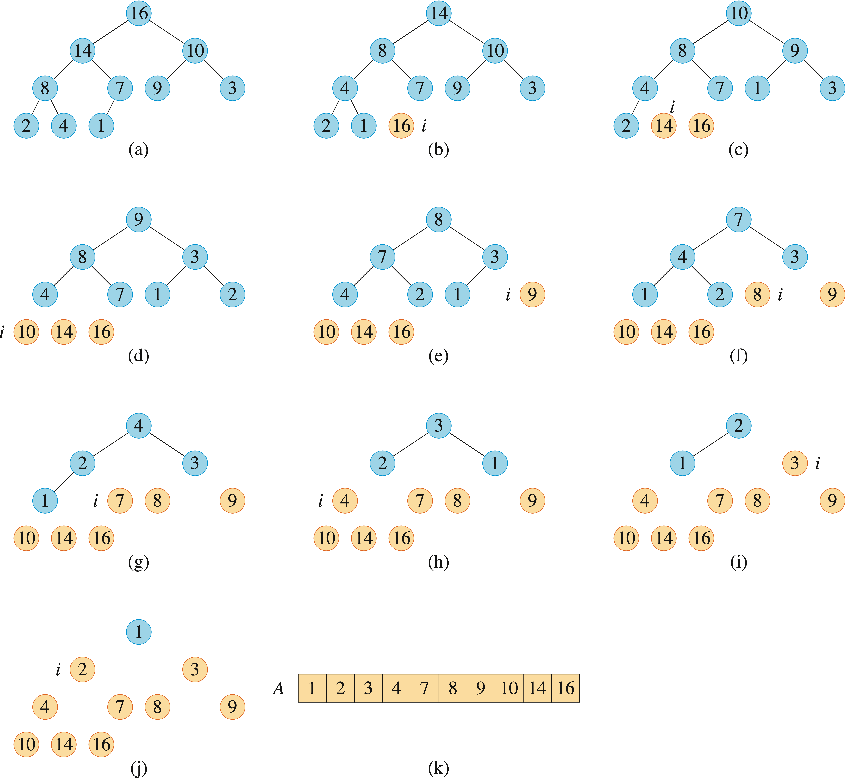
\includegraphics[width=0.7\textwidth]{Figure 6.4.pdf}
\caption{Execução Heap-Sort}
\end{figure}

\begin{theorem}
\textsc{Heapsort} ordena um arranjo de $n$ elementos em tempo $O(n\lg n)$
no pior caso.
\end{theorem}

\begin{proof}
A chamada inicial a \textsc{Build-Max-Heap} custa $O(n)$
(Teorema~\ref{teo:build-heap}). O laço executa $n-1$ iterações; cada
iteração faz trabalho $\Theta(1)$ mais uma chamada a \textsc{Max-Heapify}
na raiz, de custo $O(\lg n)$ (Proposição~\ref{prop:heapify}). Total:
\[
  T(n) = O(n) + (n-1)\cdot O(\lg n) = O(n\lg n). \qedhere
\]
\end{proof}

\paragraph{Corretude.} O invariante do laço é: no início de cada iteração,
o subarranjo $A[i+1\mathinner{.\,.} n]$ contém os $n - i$ maiores elementos em
ordem ordenada, e $A[1\mathinner{.\,.} i]$ é um max-heap. A troca coloca o maior
de $A[1\mathinner{.\,.} i]$ em $A[i]$, e \textsc{Max-Heapify} restaura a propriedade
sobre $A[1\mathinner{.\,.} i-1]$. No fim, $i = 1$ e todo o arranjo está ordenado.

\begin{example}
Considere $A = [4, 1, 3, 2, 16, 9, 10, 14, 8, 7]$. Após
\textsc{Build-Max-Heap}, $A = [16, 14, 10, 8, 7, 9, 3, 2, 4, 1]$. As
iterações subsequentes vão ``drenando'' o máximo para o final do arranjo,
produzindo a ordem crescente.
\end{example}

\subsection{Filas de prioridade}
 
Uma das aplicações mais importantes do heap é a implementação de
\impt{filas de prioridade}, uma estrutura de dados abstrata extremamente
útil em algoritmos de escalonamento de tarefas, simulações dirigidas por
eventos, algoritmos de grafos (Dijkstra, Prim), e muitas outras
aplicações.
 
\begin{definition}[Fila de prioridade]
Uma \impt{fila de prioridade} é uma estrutura de dados que mantém um
conjunto $S$ de elementos, cada um associado a uma \textbf{chave} (valor
numérico). Há duas variantes:
\begin{itemize}
  \item \impt{Fila de prioridade máxima}: suporta operações em que o
    elemento de \textbf{maior} chave tem prioridade.
  \item \impt{Fila de prioridade mínima}: análoga, com o elemento de
    \textbf{menor} chave.
\end{itemize}
\end{definition}
 
Nesta seção tratamos da variante \textbf{máxima}, implementada sobre um
max-heap. A variante mínima é obtida por simetria, usando um min-heap.
 
\paragraph{Operações.} Uma fila de prioridade máxima suporta:
\begin{itemize}
  \item \textsc{Maximum}$(S)$: retorna o elemento de $S$ com maior chave.
  \item \textsc{Extract-Max}$(S)$: remove e retorna o elemento de $S$ com
    maior chave.
  \item \textsc{Increase-Key}$(S, x, k)$: aumenta a chave do elemento $x$
    para o novo valor $k$ (que se assume $\ge$ chave atual).
  \item \textsc{Insert}$(S, x)$: insere $x$ em $S$.
\end{itemize}
 
\ntc{Na prática}, os elementos costumam ser \textit{handles} para objetos
externos (tarefas, eventos, vértices), e a chave é uma propriedade
numérica (prioridade, tempo de chegada, distância). A fila de prioridade
ordena logicamente esses elementos por chave, sem precisar de um
\textit{sort} global.
 
\subsubsection{\textsc{Heap-Maximum}}
 
Trivial: em um max-heap, o maior elemento está na raiz.
 
\begin{algorithm}[H]
\caption{\textsc{Heap-Maximum}$(A)$}
\begin{algorithmic}[1]
\State \Return $A[1]$
\end{algorithmic}
\end{algorithm}
 
Tempo: $\Theta(1)$.
 
\subsubsection{\textsc{Heap-Extract-Max}}
 
Para extrair o máximo, devolvemos $A[1]$, mas precisamos manter a
propriedade de heap. A ideia é colocar o último elemento na raiz e
descer com \textsc{Max-Heapify}.
 
\begin{algorithm}[H]
\caption{\textsc{Heap-Extract-Max}$(A)$}
\begin{algorithmic}[1]
\If{$A.\text{heap-size} < 1$}
  \State \textbf{erro} ``heap underflow''
\EndIf
\State $\textit{max} \gets A[1]$
\State $A[1] \gets A[A.\text{heap-size}]$
\State $A.\text{heap-size} \gets A.\text{heap-size} - 1$
\State \textsc{Max-Heapify}$(A, 1)$
\State \Return \textit{max}
\end{algorithmic}
\end{algorithm}
 
\begin{proposition}
\textsc{Heap-Extract-Max} executa em tempo $O(\lg n)$.
\end{proposition}
 
\begin{proof}
Todo o trabalho fora da chamada a \textsc{Max-Heapify} é $\Theta(1)$. A
chamada custa $O(\lg n)$ pela Proposição~\ref{prop:heapify}.
\end{proof}
 
\paragraph{Corretude.} Antes da chamada a \textsc{Max-Heapify}, a raiz
$A[1]$ pode violar a propriedade de max-heap, mas ambas as subárvores de
$A[1]$ \textit{continuam} sendo max-heaps --- nenhuma operação anterior
as modificou. Essa é exatamente a pré-condição de \textsc{Max-Heapify},
que restaura a propriedade em $O(\lg n)$.
 
\subsubsection{\textsc{Heap-Increase-Key}}
 
Aumentar a chave de um elemento pode violar a propriedade de max-heap
apenas ``para cima'' --- o novo valor pode exceder o valor do pai. A
operação percorre o caminho até a raiz, trocando com o pai sempre que
necessário.
 
\begin{algorithm}[H]
\caption{\textsc{Heap-Increase-Key}$(A, i, \textit{key})$}
\begin{algorithmic}[1]
\If{$\textit{key} < A[i]$}
  \State \textbf{erro} ``nova chave é menor que a atual''
\EndIf
\State $A[i] \gets \textit{key}$
\While{$i > 1$ \textbf{e} $A[\textsc{Parent}(i)] < A[i]$}
  \State troca $A[i] \leftrightarrow A[\textsc{Parent}(i)]$
  \State $i \gets \textsc{Parent}(i)$
\EndWhile
\end{algorithmic}
\end{algorithm}
 
\paragraph{Invariante do laço.} No início de cada iteração, o arranjo
$A[1\mathinner{.\,.} A.\text{heap-size}]$ satisfaz a propriedade de max-heap,
\textbf{exceto possivelmente} pelo par $(A[i], A[\textsc{Parent}(i)])$,
onde $A[i]$ pode ser maior que $A[\textsc{Parent}(i)]$.
 
\textbf{Inicialização.} Antes da primeira iteração, a única posição
alterada foi $A[i]$. Como as subárvores de $A[i]$ continuam max-heaps
(seus valores não mudaram) e todos os outros pares pai--filho também
permanecem corretos, a única possível violação é entre $A[i]$ e seu pai.
 
\textbf{Manutenção.} Se $A[\textsc{Parent}(i)] < A[i]$, a troca corrige a
violação local. Mas agora o valor de $A[i]$ (antigo $A[\textsc{Parent}(i)]$)
pode ser menor que o outro filho do pai? \textbf{Não}: o outro filho já
era $\le A[\textsc{Parent}(i)]$ antes da troca, e $A[\textsc{Parent}(i)]$
recebeu o valor antigo de $A[i]$, que é maior ainda. Logo, a única
possível violação nova está entre o novo $A[\textsc{Parent}(i)]$ e
\textit{seu} pai --- e é exatamente o que o novo valor de $i$
(\textsc{Parent}(i)$) $ aponta.
 
\textbf{Término.} Ou $i = 1$ (chegamos na raiz, nada acima para
violar), ou $A[\textsc{Parent}(i)] \ge A[i]$ (a propriedade é satisfeita
localmente, e por indução em toda a árvore).
 
\begin{proposition}
\textsc{Heap-Increase-Key} executa em tempo $O(\lg n)$.
\end{proposition}
 
\begin{proof}
Cada iteração do laço sobe um nível na árvore. Como a altura é
$\lfloor \lg n \rfloor$ (Lema~\ref{lem:altura}), o laço executa no máximo
$\lfloor \lg n \rfloor$ iterações, cada uma em tempo $\Theta(1)$.
\end{proof}
 
\subsubsection{\textsc{Max-Heap-Insert}}
 
Inserir um novo elemento com chave $k$ é fácil de implementar
reutilizando \textsc{Heap-Increase-Key}: colocamos $-\infty$ na nova
posição (última folha) e então ``aumentamos'' essa chave para $k$.
 
\begin{algorithm}[H]
\caption{\textsc{Max-Heap-Insert}$(A, \textit{key})$}
\begin{algorithmic}[1]
\State $A.\text{heap-size} \gets A.\text{heap-size} + 1$
\State $A[A.\text{heap-size}] \gets -\infty$
\State \textsc{Heap-Increase-Key}$(A, A.\text{heap-size}, \textit{key})$
\end{algorithmic}
\end{algorithm}
 
\begin{proposition}
\textsc{Max-Heap-Insert} executa em tempo $O(\lg n)$.
\end{proposition}
 
\begin{proof}
As duas primeiras linhas custam $\Theta(1)$; a chamada a
\textsc{Heap-Increase-Key} custa $O(\lg n)$.
\end{proof}
 
\ntc{Truque pedagógico:} usar $-\infty$ como chave inicial garante que
a propriedade de max-heap vale trivialmente antes da chamada a
\textsc{Heap-Increase-Key} (qualquer valor é maior), e assim a operação
de subida está sempre bem definida.
 
\begin{example}
Sobre o heap $A = [16, 14, 10, 8, 7, 9, 3, 2, 4, 1]$, executar
\textsc{Max-Heap-Insert}$(A, 15)$:
\begin{enumerate}
  \item Coloca $-\infty$ em $A[11]$: $[16, 14, 10, 8, 7, 9, 3, 2, 4, 1, -\infty]$.
  \item \textsc{Heap-Increase-Key}$(A, 11, 15)$: aumenta para $15$.
  \item Sobe: $A[11] = 15 > A[5] = 7$ $\Rightarrow$ troca.
  \item Sobe: $A[5] = 15 > A[2] = 14$ $\Rightarrow$ troca.
  \item Sobe: $A[2] = 15 < A[1] = 16$ $\Rightarrow$ para.
\end{enumerate}
Resultado: $[16, 15, 10, 8, 14, 9, 3, 2, 4, 1, 7]$.
\end{example}
 
\subsubsection{Resumo das operações}
 
\begin{center}
\begin{tabular}{l c l}
\toprule
\textbf{Operação} & \textbf{Tempo} & \textbf{Mecanismo} \\
\midrule
\textsc{Heap-Maximum}        & $\Theta(1)$   & Lê raiz \\
\textsc{Heap-Extract-Max}    & $O(\lg n)$    & Troca e desce (\textsc{Max-Heapify}) \\
\textsc{Heap-Increase-Key}   & $O(\lg n)$    & Sobe trocando com pai \\
\textsc{Max-Heap-Insert}     & $O(\lg n)$    & Inserção + \textsc{Increase-Key} \\
\bottomrule
\end{tabular}
\end{center}
 
\ntc{Operação relacionada:} \textsc{Heap-Delete}$(A, i)$, que remove o
elemento $A[i]$, também pode ser feita em $O(\lg n)$ (Exercício 6.5-8
do CLRS). A ideia é substituir $A[i]$ pelo último elemento e chamar
\textsc{Max-Heapify} ou \textsc{Heap-Increase-Key}, dependendo da
comparação.
 
\subsubsection{Aplicações}
 
Filas de prioridade são ubíquas. Alguns usos clássicos:
\begin{itemize}
  \item \impt{Escalonamento em sistemas operacionais}: processos são
    extraídos em ordem decrescente de prioridade.
  \item \impt{Simulação dirigida por eventos}: eventos futuros são
    armazenados em uma fila de prioridade mínima pela chave ``tempo de
    ocorrência''; o simulador sempre extrai o próximo evento.
  \item \impt{Algoritmo de Dijkstra} (caminhos mínimos em grafos): usa
    uma fila de prioridade mínima de vértices, com chave = distância
    estimada à origem, e executa \textsc{Decrease-Key} ao relaxar
    arestas.
  \item \impt{Algoritmo de Prim} (árvore geradora mínima): estrutura
    idêntica à de Dijkstra, adaptada para peso mínimo ligando a árvore.
  \item \impt{Codificação de Huffman}: usa uma fila de prioridade
    mínima para construir iterativamente a árvore de códigos a partir
    das frequências.
\end{itemize}
 

% =====================================================================
\section{Quicksort}

\subsection{Descrição}

O quicksort segue o paradigma \impt{divisão e conquista}, com a divisão
feita por \textbf{particionamento em torno de um pivô}.

\begin{itemize}
  \item \textbf{Divide:} escolhe um pivô $x \in A[p\mathinner{.\,.} r]$ e particiona
    o arranjo em dois subarranjos (possivelmente vazios) $A[p\mathinner{.\,.} q-1]$
    e $A[q+1\mathinner{.\,.} r]$ tais que todo elemento do primeiro é $\le x$ e todo
    elemento do segundo é $\ge x$. Posição $q$ é o índice final do pivô.
  \item \textbf{Conquista:} ordena recursivamente $A[p\mathinner{.\,.} q-1]$ e
    $A[q+1\mathinner{.\,.} r]$.
  \item \textbf{Combina:} nada a fazer --- o arranjo já está ordenado.
\end{itemize}

\begin{algorithm}[H]
\caption{\textsc{Quicksort}$(A, p, r)$}
\begin{algorithmic}[1]
\If{$p < r$}
  \State $q \gets \textsc{Partition}(A, p, r)$
  \State \textsc{Quicksort}$(A, p, q-1)$
  \State \textsc{Quicksort}$(A, q+1, r)$
\EndIf
\end{algorithmic}
\end{algorithm}

\subsection{\textsc{Partition}: o núcleo do algoritmo}

Usamos o esquema de \impt{Lomuto}, como no CLRS: escolhe-se $A[r]$ como
pivô e mantém-se um índice $i$ que separa elementos $\le x$ dos $> x$.

\begin{algorithm}[H]
\caption{\textsc{Partition}$(A, p, r)$}
\begin{algorithmic}[1]
\State $x \gets A[r]$
\State $i \gets p - 1$
\For{$j \gets p$ \textbf{até} $r - 1$}
  \If{$A[j] \le x$}
    \State $i \gets i + 1$
    \State troca $A[i] \leftrightarrow A[j]$
  \EndIf
\EndFor
\State troca $A[i+1] \leftrightarrow A[r]$
\State \Return $i + 1$
\end{algorithmic}
\end{algorithm}

\paragraph{Invariante de laço.} No início de cada iteração do \texttt{for}:
\begin{enumerate}
  \item[(i)] Se $p \le k \le i$, então $A[k] \le x$.
  \item[(ii)] Se $i+1 \le k \le j-1$, então $A[k] > x$.
  \item[(iii)] $A[r] = x$.
\end{enumerate}

\textbf{Inicialização.} Antes da primeira iteração, $i = p-1$ e $j = p$:
as faixas (i) e (ii) estão vazias; (iii) vale pela atribuição.

\textbf{Manutenção.} Considere a iteração com valor $j$. Se $A[j] > x$,
incrementamos $j$ e $(i,j-1)$ passa a conter $A[j]$, preservando (ii).
Se $A[j] \le x$, incrementamos $i$, trocamos $A[i] \leftrightarrow A[j]$ e
incrementamos $j$: o novo $A[i] \le x$ (preservando (i)) e o elemento que
estava em $A[i]$ --- que era $> x$ --- move-se para $A[j-1]$ (preservando (ii)).

\textbf{Término.} $j = r$. Pelo invariante, $A[p\mathinner{.\,.} i] \le x$ e
$A[i+1\mathinner{.\,.} r-1] > x$. A troca final coloca o pivô na posição $i+1$, que
é portanto o índice devolvido.

\begin{proposition}
\textsc{Partition} executa em tempo $\Theta(n)$, onde $n = r - p + 1$.
\end{proposition}

\begin{proof}
O laço \textbf{for} itera $n - 1$ vezes; cada iteração faz trabalho
$\Theta(1)$.
\end{proof}

\subsection{Análise: pior caso}

\begin{theorem}\label{teo:qsort-pior}
O tempo de pior caso do quicksort sobre $n$ elementos é $\Theta(n^2)$.
\end{theorem}

O pior caso ocorre quando o particionamento é \impt{maximamente
desbalanceado} em cada chamada --- por exemplo, quando o arranjo já está
ordenado (ou em ordem inversa), de modo que o pivô é sempre o maior (ou
menor) elemento. A partição produz então um lado com $n-1$ elementos e
outro vazio.

\begin{proof}[Demonstração]
Seja $T(n)$ o tempo de pior caso. Existe particionamento maximamente
desbalanceado (mostrado acima), produzindo a recorrência
\[
  T(n) = T(n-1) + T(0) + \Theta(n) = T(n-1) + \Theta(n),
\]
cuja solução, por expansão, é
\[
  T(n) = \sum_{k=1}^{n} \Theta(k) = \Theta(n^2).
\]
Para o limite superior, mostramos por indução --- usando o método da
substituição --- que $T(n) = O(n^2)$. Suponha $T(k) \le c k^2$ para todo
$k < n$. Como o particionamento produz dois subproblemas de tamanhos
$q$ e $n - q - 1$ com $0 \le q \le n-1$, e como $q^2 + (n-q-1)^2$ é
maximizado nos extremos $q \in \{0, n-1\}$, temos
\[
  T(n) \le \max_{0 \le q \le n-1}\{ c q^2 + c(n-q-1)^2 \} + \Theta(n)
       \le c(n-1)^2 + \Theta(n)
       \le c n^2,
\]
para $c$ suficientemente grande. Logo $T(n) = \Theta(n^2)$.
\end{proof}

\subsection{Análise: melhor caso e caso balanceado}

\paragraph{Melhor caso.} Se o particionamento é perfeitamente balanceado
em cada chamada, $T(n) = 2\, T(n/2) + \Theta(n)$, e pelo método mestre
(caso 2), $T(n) = \Theta(n\lg n)$.

\paragraph{Particionamento ``razoável''.} O resultado mais interessante
do CLRS é que mesmo partições \textit{consistentemente desbalanceadas} ---
mas em proporção constante --- ainda dão $O(n\lg n)$:

\begin{proposition}
Se todo particionamento divide o arranjo em frações $\alpha$ e $1 - \alpha$
com $0 < \alpha \le 1/2$ constante, então $T(n) = O(n\lg n)$.
\end{proposition}

\begin{proof}[Ideia]
A recorrência é $T(n) = T(\alpha n) + T((1-\alpha) n) + \Theta(n)$. A
árvore de recursão tem profundidade $\Theta(\lg n)$ (dominada pelo ramo
mais longo, de tamanho $((1-\alpha))^k n$, que atinge 1 em
$\log_{1/(1-\alpha)} n = \Theta(\lg n)$ passos) e cada nível custa $O(n)$
\ntc{(lembre: o custo em um nível é a soma dos tamanhos, e essa soma não
aumenta com a profundidade)}. Logo $T(n) = O(n\lg n)$.
\end{proof}

\paragraph{Intuição.} Particionamentos bons e ruins se alternam de forma
natural em entradas aleatórias. Um nível ``ruim'' seguido de um ``bom''
dá o mesmo efeito de dois níveis ``razoáveis''. Isso motiva a análise
probabilística.

\subsection{Quicksort aleatorizado}

Para evitar que entradas adversárias produzam o pior caso sistematicamente,
escolhemos o pivô aleatoriamente:

\begin{algorithm}[H]
\caption{\textsc{Randomized-Partition}$(A, p, r)$}
\begin{algorithmic}[1]
\State $i \gets \textsc{Random}(p, r)$
\State troca $A[r] \leftrightarrow A[i]$
\State \Return \textsc{Partition}$(A, p, r)$
\end{algorithmic}
\end{algorithm}

O \textsc{Randomized-Quicksort} simplesmente chama
\textsc{Randomized-Partition} no lugar de \textsc{Partition}. O pivô passa
a ser uniformemente distribuído entre os elementos do subarranjo.

\subsection{Análise do caso médio}

\begin{theorem}\label{teo:qsort-medio}
O tempo esperado do \textsc{Randomized-Quicksort} sobre uma entrada de
$n$ elementos distintos é $O(n\lg n)$.
\end{theorem}

A prova segue a técnica de \impt{contagem de comparações}, central no
CLRS.

\paragraph{Observação-chave.} O tempo total é dominado pelo número de
comparações realizadas em todas as chamadas a \textsc{Partition}. Mais
precisamente, se $X$ é o número total de comparações, então o tempo é
$O(n + X)$.

\paragraph{Indicadores.} Renomeie os elementos de $A$ como $z_1 < z_2 <
\dots < z_n$ (estatísticas de ordem). Para $i < j$, seja
\[
  X_{ij} = \mathbb{I}\{z_i \text{ é comparado a } z_j\}.
\]
Então $X = \sum_{i<j} X_{ij}$. Pela linearidade,
\[
  \mathbb{E}[X] = \sum_{i=1}^{n-1}\sum_{j=i+1}^{n} \Pr[z_i\text{ é comparado a }z_j].
\]

\begin{lemma}\label{lem:prob-comparacao}
$\Pr[z_i\text{ é comparado a }z_j] = \dfrac{2}{j - i + 1}$.
\end{lemma}

\begin{proof}
$z_i$ e $z_j$ só podem ser comparados \textbf{em uma chamada a
\textsc{Partition} cujo intervalo contenha ambos}. Considere o conjunto
$Z_{ij} = \{z_i, z_{i+1}, \dots, z_j\}$, de cardinalidade $j - i + 1$. O
primeiro elemento de $Z_{ij}$ a ser escolhido como pivô separa o caso
em dois cenários:
\begin{itemize}
  \item Se o pivô é $z_i$ ou $z_j$, então $z_i$ e $z_j$ \textbf{são}
    comparados (pivô contra não-pivô).
  \item Se o pivô é algum $z_k$ com $i < k < j$, então $z_i$ e $z_j$
    vão para subarranjos distintos --- e \textbf{nunca mais} serão
    comparados.
\end{itemize}
Como cada elemento de $Z_{ij}$ tem igual probabilidade de ser o primeiro
pivô escolhido em $Z_{ij}$ (propriedade da escolha uniforme), a
probabilidade de o pivô inicial ser $z_i$ ou $z_j$ é
$\dfrac{2}{j - i + 1}$.
\end{proof}

\begin{proof}[Prova do Teorema~\ref{teo:qsort-medio}]
Usando o Lema~\ref{lem:prob-comparacao},
\[
  \mathbb{E}[X]
  = \sum_{i=1}^{n-1} \sum_{j=i+1}^{n} \frac{2}{j - i + 1}
  = \sum_{i=1}^{n-1} \sum_{k=2}^{n - i + 1} \frac{2}{k}
  \;\le\; \sum_{i=1}^{n-1} 2 H_n
  = O(n\lg n),
\]
onde $H_n = \sum_{k=1}^{n} 1/k = \Theta(\lg n)$ é o $n$-ésimo número
harmônico. Logo $\mathbb{E}[X] = O(n\lg n)$, e o tempo total esperado é
$O(n + n\lg n) = O(n\lg n)$.
\end{proof}

\begin{remark}
A análise não depende de nenhuma hipótese sobre a entrada: a
aleatoriedade está no algoritmo, não nos dados. Este é o grande ganho
conceitual do quicksort aleatorizado.
\end{remark}

% =====================================================================
\section{Comparação com os outros métodos}

\subsection{Panorama}

A tabela abaixo resume as características principais dos quatro métodos
vistos no curso:

\begin{center}
\small
\begin{tabularx}{\textwidth}{l c c c c X}
\toprule
\textbf{Algoritmo} & \textbf{Melhor caso} & \textbf{Pior caso} & \textbf{Caso médio} & \textbf{In place?} & \textbf{Estável?} \\
\midrule
Insertion sort    & $\Theta(n)$       & $\Theta(n^2)$   & $\Theta(n^2)$   & Sim  & Sim \\
Merge sort        & $\Theta(n\lg n)$  & $\Theta(n\lg n)$& $\Theta(n\lg n)$& Não & Sim \\
Heapsort          & $\Theta(n\lg n)$\footnotemark & $\Theta(n\lg n)$& $\Theta(n\lg n)$ & Sim & Não \\
Quicksort (aleat.)& $\Theta(n\lg n)$  & $\Theta(n^2)$   & $\Theta(n\lg n)$ (esp.) & Sim & Não \\
\bottomrule
\end{tabularx}
\end{center}
\footnotetext{Rigorosamente, $\Omega(n)$ se todos os elementos são iguais; $\Theta(n\lg n)$ no caso genérico.}

\subsection{Quando usar cada um?}

\paragraph{\impt{Insertion sort}.} Apesar de $\Theta(n^2)$, é
extraordinariamente rápido para $n$ pequeno (constante $< 10$) --- por
isso é usado como \textit{caso base} em implementações híbridas de
merge/quicksort. Também é o melhor para arranjos \textit{quase
ordenados}: $\Theta(n + d)$, onde $d$ é o número de inversões.

\paragraph{\impt{Merge sort}.} Escolha natural quando (i) estabilidade é
essencial, (ii) os dados não cabem em memória (\textit{external sort}),
ou (iii) a entrada está em listas encadeadas. Custo: precisa de
$\Theta(n)$ memória adicional.

\paragraph{\impt{Heapsort}.} Garantia rígida de $O(n\lg n)$ \textit{in
place} --- interessante em sistemas de tempo real onde pior caso
importa. Na prática, porém, costuma ser $\sim 2\times$ mais lento que o
quicksort em entradas aleatórias, por causa do padrão de acesso à
memória (pouca localidade de cache).

\paragraph{\impt{Quicksort aleatorizado}.} Padrão de fato para dados em
memória. Constantes pequenas, excelente localidade (o particionamento
varre o arranjo linearmente), e pior caso raríssimo em prática. É o
algoritmo por trás de \texttt{qsort} da libc, \texttt{std::sort} do C++
(híbrido com heapsort --- \textit{introsort}), e das implementações
de \texttt{sort()} em Java e Python (Timsort, que é um híbrido com merge
sort).

\subsection{Diagrama das recorrências}

\begin{center}
\begin{tikzpicture}[
  node distance=1.1cm,
  box/.style={draw, rounded corners, align=center, inner sep=5pt, minimum width=4.5cm}
]
\node[box] (ms) {Merge sort\\[2pt] $T(n) = 2T(n/2) + \Theta(n)$\\[2pt] $\Rightarrow \Theta(n\lg n)$};
\node[box, right=of ms] (hs) {Heapsort\\[2pt] $\textsc{Build} + (n-1)\cdot O(\lg n)$\\[2pt] $\Rightarrow O(n\lg n)$};
\node[box, below=of ms] (qs-worst) {Quicksort pior\\[2pt] $T(n) = T(n-1) + \Theta(n)$\\[2pt] $\Rightarrow \Theta(n^2)$};
\node[box, below=of hs] (qs-avg) {Quicksort médio\\[2pt] $\mathbb{E}[X] = O(n\lg n)$\\[2pt] via comparações};
\end{tikzpicture}
\end{center}

% =====================================================================
\section{Exercícios sugeridos do CLRS}

Para fixação, recomendam-se os seguintes exercícios do \citet{cormen2009}:
\begin{itemize}
  \item \textbf{Heapsort:} 6.1-1, 6.1-2, 6.2-5 (iterativo), 6.3-3, 6.4-2,
    6.5-7.
  \item \textbf{Quicksort:} 7.1-1, 7.1-2, 7.2-2, 7.2-3, 7.3-1, 7.4-2,
    7.4-5 (combinação com insertion sort).
\end{itemize}

\bibliographystyle{apalike}
\begin{thebibliography}{1}
\bibitem[Cormen et al.(2009)]{cormen2009}
Cormen, T.~H., Leiserson, C.~E., Rivest, R.~L., \& Stein, C. (2009).
\newblock \emph{Introduction to Algorithms} (3rd ed.).
\newblock MIT Press.
\end{thebibliography}

\end{document}
